\documentclass[tikz, border=1mm]{standalone}
\begin{document}

\tikzset{every picture/.style={line width=0.75pt}} %set default line width to 0.75pt

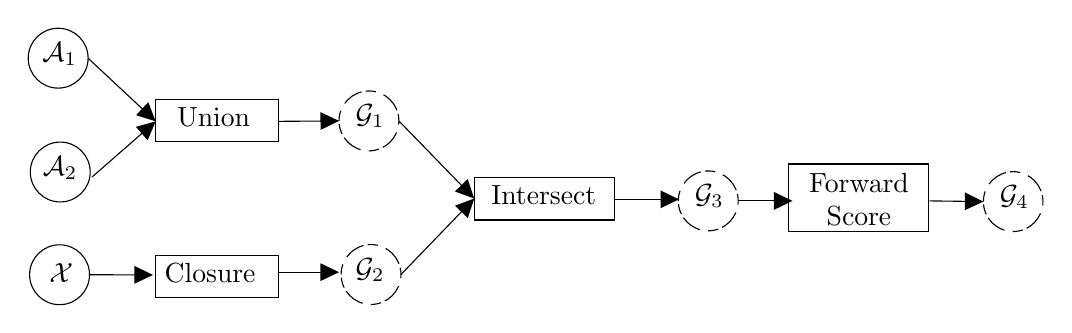
\begin{tikzpicture}[x=0.75pt,y=0.75pt,yscale=-1,xscale=1]
%uncomment if require: \path (0,400); %set diagram left start at 0, and has height of 400

%Shape: Rectangle [id:dp3397381853835959]
\draw   (113.67,146.01) -- (172.67,146.01) -- (172.67,166.12) -- (113.67,166.12) -- cycle ;
%Shape: Rectangle [id:dp33192079042323686]
\draw   (267.13,183.21) -- (334.8,183.21) -- (334.8,203.87) -- (267.13,203.87) -- cycle ;
%Shape: Rectangle [id:dp4285669013568696]
\draw   (418.47,176.87) -- (486.13,176.87) -- (486.13,209.53) -- (418.47,209.53) -- cycle ;

%Shape: Rectangle [id:dp27723208562192236]
\draw   (113.67,220.89) -- (173,220.89) -- (173,241) -- (113.67,241) -- cycle ;
%Straight Lines [id:da9103743349863969]
\draw    (83,183.15) -- (111.41,158.32) ;
\draw [shift={(113.67,156.34)}, rotate = 498.84] [fill={rgb, 255:red, 0; green, 0; blue, 0 }  ][line width=0.08]  [draw opacity=0] (8.93,-4.29) -- (0,0) -- (8.93,4.29) -- cycle    ;
%Straight Lines [id:da6425774963316973]
\draw    (173,229.01) -- (198.98,229.01) ;
\draw [shift={(201.98,229.01)}, rotate = 180] [fill={rgb, 255:red, 0; green, 0; blue, 0 }  ][line width=0.08]  [draw opacity=0] (8.93,-4.29) -- (0,0) -- (8.93,4.29) -- cycle    ;
%Straight Lines [id:da05623583706962054]
\draw    (231.82,230.13) -- (265.05,195.7) ;
\draw [shift={(267.13,193.54)}, rotate = 493.98] [fill={rgb, 255:red, 0; green, 0; blue, 0 }  ][line width=0.08]  [draw opacity=0] (8.93,-4.29) -- (0,0) -- (8.93,4.29) -- cycle    ;
%Straight Lines [id:da8206690048250029]
\draw    (81.09,125.91) -- (111.47,154.3) ;
\draw [shift={(113.67,156.34)}, rotate = 223.06] [fill={rgb, 255:red, 0; green, 0; blue, 0 }  ][line width=0.08]  [draw opacity=0] (8.93,-4.29) -- (0,0) -- (8.93,4.29) -- cycle    ;
%Straight Lines [id:da476011248422078]
\draw    (486.47,194.67) -- (509.44,194.96) ;
\draw [shift={(512.44,195)}, rotate = 180.74] [fill={rgb, 255:red, 0; green, 0; blue, 0 }  ][line width=0.08]  [draw opacity=0] (8.93,-4.29) -- (0,0) -- (8.93,4.29) -- cycle    ;
%Straight Lines [id:da4946727022220827]
\draw    (335.13,193.93) -- (362.8,193.93) ;
\draw [shift={(365.8,193.93)}, rotate = 180] [fill={rgb, 255:red, 0; green, 0; blue, 0 }  ][line width=0.08]  [draw opacity=0] (8.93,-4.29) -- (0,0) -- (8.93,4.29) -- cycle    ;
%Shape: Circle [id:dp2569559403283066]
\draw   (53.24,180.75) .. controls (53.24,172.78) and (59.7,166.33) .. (67.67,166.33) .. controls (75.63,166.33) and (82.09,172.78) .. (82.09,180.75) .. controls (82.09,188.72) and (75.63,195.18) .. (67.67,195.18) .. controls (59.7,195.18) and (53.24,188.72) .. (53.24,180.75) -- cycle ;
%Shape: Circle [id:dp10905410543312533]
\draw   (52.24,125.91) .. controls (52.24,117.94) and (58.7,111.48) .. (66.67,111.48) .. controls (74.63,111.48) and (81.09,117.94) .. (81.09,125.91) .. controls (81.09,133.88) and (74.63,140.33) .. (66.67,140.33) .. controls (58.7,140.33) and (52.24,133.88) .. (52.24,125.91) -- cycle ;
%Shape: Circle [id:dp27289812346327014]
\draw   (52.91,230.24) .. controls (52.91,222.27) and (59.37,215.82) .. (67.33,215.82) .. controls (75.3,215.82) and (81.76,222.27) .. (81.76,230.24) .. controls (81.76,238.21) and (75.3,244.67) .. (67.33,244.67) .. controls (59.37,244.67) and (52.91,238.21) .. (52.91,230.24) -- cycle ;
%Shape: Circle [id:dp2507568180420352]
\draw  [dash pattern={on 3.75pt off 3pt on 7.5pt off 1.5pt}] (201.98,156.13) .. controls (201.98,148.17) and (208.43,141.71) .. (216.4,141.71) .. controls (224.37,141.71) and (230.82,148.17) .. (230.82,156.13) .. controls (230.82,164.1) and (224.37,170.56) .. (216.4,170.56) .. controls (208.43,170.56) and (201.98,164.1) .. (201.98,156.13) -- cycle ;
%Shape: Circle [id:dp8458980581712332]
\draw  [dash pattern={on 3.75pt off 3pt on 7.5pt off 1.5pt}] (202.98,230.13) .. controls (202.98,222.17) and (209.43,215.71) .. (217.4,215.71) .. controls (225.37,215.71) and (231.82,222.17) .. (231.82,230.13) .. controls (231.82,238.1) and (225.37,244.56) .. (217.4,244.56) .. controls (209.43,244.56) and (202.98,238.1) .. (202.98,230.13) -- cycle ;
%Shape: Circle [id:dp7494739065578262]
\draw  [dash pattern={on 3.75pt off 3pt on 7.5pt off 1.5pt}] (365.44,194.67) .. controls (365.44,186.7) and (371.9,180.24) .. (379.87,180.24) .. controls (387.83,180.24) and (394.29,186.7) .. (394.29,194.67) .. controls (394.29,202.63) and (387.83,209.09) .. (379.87,209.09) .. controls (371.9,209.09) and (365.44,202.63) .. (365.44,194.67) -- cycle ;
%Shape: Ellipse [id:dp34645516680948507]
\draw  [dash pattern={on 3.75pt off 3pt on 7.5pt off 1.5pt}] (512.44,195) .. controls (512.44,187.03) and (518.86,180.58) .. (526.79,180.58) .. controls (534.71,180.58) and (541.13,187.03) .. (541.13,195) .. controls (541.13,202.97) and (534.71,209.42) .. (526.79,209.42) .. controls (518.86,209.42) and (512.44,202.97) .. (512.44,195) -- cycle ;
%Straight Lines [id:da5751831342851284]
\draw    (394.29,194.67) -- (417.47,194.67) ;
\draw [shift={(420.47,194.67)}, rotate = 180] [fill={rgb, 255:red, 0; green, 0; blue, 0 }  ][line width=0.08]  [draw opacity=0] (8.93,-4.29) -- (0,0) -- (8.93,4.29) -- cycle    ;
%Straight Lines [id:da5888997290383744]
\draw    (173,156.34) -- (198.98,156.16) ;
\draw [shift={(201.98,156.13)}, rotate = 539.5799999999999] [fill={rgb, 255:red, 0; green, 0; blue, 0 }  ][line width=0.08]  [draw opacity=0] (8.93,-4.29) -- (0,0) -- (8.93,4.29) -- cycle    ;
%Straight Lines [id:da44882081298177434]
\draw    (230.82,156.13) -- (265.04,191.39) ;
\draw [shift={(267.13,193.54)}, rotate = 225.86] [fill={rgb, 255:red, 0; green, 0; blue, 0 }  ][line width=0.08]  [draw opacity=0] (8.93,-4.29) -- (0,0) -- (8.93,4.29) -- cycle    ;
%Straight Lines [id:da7440962899149539]
\draw    (81.76,230.24) -- (109.33,230.33) ;
\draw [shift={(112.33,230.34)}, rotate = 180.19] [fill={rgb, 255:red, 0; green, 0; blue, 0 }  ][line width=0.08]  [draw opacity=0] (8.93,-4.29) -- (0,0) -- (8.93,4.29) -- cycle    ;

% Text Node
\draw (424.47,179.87) node [anchor=north west][inner sep=0.75pt]   [align=left] {\begin{minipage}[lt]{40.13pt}\setlength\topsep{0pt}
\begin{center}
Forward\\Score
\end{center}

\end{minipage}};
% Text Node
\draw (58.03,172.17) node [anchor=north west][inner sep=0.75pt]    {$\mathcal{A}_{2}$};
% Text Node
\draw (57.83,116.93) node [anchor=north west][inner sep=0.75pt]    {$\mathcal{A}_{1}$};
% Text Node
\draw (61.2,223.47) node [anchor=north west][inner sep=0.75pt]    {$\mathcal{X}$};
% Text Node
\draw (274.13,186.2) node [anchor=north west][inner sep=0.75pt]   [align=left] {Intersect};
% Text Node
\draw (208.7,147.07) node [anchor=north west][inner sep=0.75pt]    {$\mathcal{G}_{1}$};
% Text Node
\draw (208.7,221.07) node [anchor=north west][inner sep=0.75pt]    {$\mathcal{G}_{2}$};
% Text Node
\draw (372.17,185.6) node [anchor=north west][inner sep=0.75pt]    {$\mathcal{G}_{3}$};
% Text Node
\draw (519.08,186.07) node [anchor=north west][inner sep=0.75pt]    {$\mathcal{G}_{4}$};
% Text Node
\draw (116.67,223.67) node [anchor=north west][inner sep=0.75pt]   [align=left] {Closure};
% Text Node
\draw (122.67,148.67) node [anchor=north west][inner sep=0.75pt]   [align=left] {Union};


\end{tikzpicture}
\end{document}

